%=============================================================================
% FairTox -- DLE-AI-202 final project report (Track 2: applied / domain research)
%
% Build:  cd report && latexmk -pdf report.tex      (or: pdflatex x2)
%
% Every number in every table comes from report/tables/*.tex, which is written by
% scripts/make_paper_tables.py from the committed analysis artefacts. Every
% figure comes from report/figures/*.pdf, written by scripts/make_paper_figures.py
% from the same artefacts. Nothing in this document is typed in by hand, so the
% paper cannot drift away from the results it reports.
%=============================================================================
\documentclass[conference]{IEEEtran}
\IEEEoverridecommandlockouts

\usepackage{cite}
\usepackage{amsmath,amssymb,amsfonts}
\usepackage{algorithm}
\usepackage{algpseudocode}
\usepackage{graphicx}
\usepackage{booktabs}
\usepackage{multirow}
\usepackage{url}
\usepackage{xcolor}
\usepackage{balance}
\usepackage[hidelinks]{hyperref}

\graphicspath{{figures/}}

% --- the four details that live in one place ---------------------------------
\newcommand{\repourl}{https://github.com/nigarrustamova/fairtox}
\newcommand{\repotag}{v1.0-final}

\begin{document}

\title{Parity, Utility and Safety Are Not Independent:\\
A Controlled Comparison of Three Bias-Mitigation\\
Families for Toxicity Classification}

% Authors are listed Surname, Given name(s), sorted alphabetically by surname,
% as the brief requires.
\author{
\IEEEauthorblockN{Aliyev, Orkhan\thanks{All authors are with the AI Academy,
National Artificial Intelligence Centre, Baku, Azerbaijan. Course DLE-AI-202,
Cohort I, 2026.}}
\IEEEauthorblockA{\textit{AI Academy}\\
Baku, Azerbaijan\\
\footnotesize
orxan.aliyev25@aiacademy.edu.az}
\and
\IEEEauthorblockN{Mirzayeva, Laman}
\IEEEauthorblockA{\textit{AI Academy}\\
Baku, Azerbaijan\\
\footnotesize
leman.mirzayeva25@aiacademy.edu.az}
\and
\IEEEauthorblockN{Rustamova, Nigar}
\IEEEauthorblockA{\textit{AI Academy}\\
Baku, Azerbaijan\\
\footnotesize
nigar.rustemova25@aiacademy.edu.az}
\and
\IEEEauthorblockN{Samadov, Nijat}
\IEEEauthorblockA{\textit{AI Academy}\\
Baku, Azerbaijan\\
\footnotesize
nicat.semedov25@aiacademy.edu.az}
}

\maketitle

\begin{abstract}
Toxicity classifiers over-flag benign text that mentions demographic groups, and
a large literature proposes fixes at three different points of the pipeline: the
data, the loss, and the decision threshold. Those fixes are almost never compared
against one another on one corpus under one recipe. We run that comparison. On
the Jigsaw Unintended Bias corpus we fine-tune DistilBERT and evaluate eight
trained configurations, plus a training-free post-processing arm, on three axes
kept deliberately separate---utility, parity, and safety---each against a
structurally controlled baseline that differs from it in exactly one thing. Identity-aware loss reweighting reduces the subgroup
false-positive-rate gap by $0.0520$ (95\% CI $[-0.0742, -0.0297]$; $8/8$ seeds;
exact sign test $p = 0.0078$) and flattens the regression of subgroup FPR on
subgroup toxic rate by $44.6\%$, but costs $0.1138$ of subgroup false-negative
rate: $2.19$ points of missed abuse per point of gap closed. Counterfactual
augmentation is a null result at two doses, and the higher dose is the more
informative one---it flattens the same shortcut by $30.9\%$ while leaving the gap
slightly worse, showing that removing the lexical shortcut is \emph{not}
sufficient to remove the disparity. Group DRO, the same objective with the human
choice removed, moves the gap $2.6\times$ the wrong way and its learned weights
explain why. Together with two hand-built controls this yields the paper's main
claim: the parity gain requires an \emph{asymmetric} weighting of the
identity-bearing non-toxic cell alone, and any objective that also raises the
identity-bearing toxic cell---chosen or learned---travels the same frontier
backwards. Code, all $38$ runs and every table:
\url{\repourl} (tag \texttt{\repotag}).
\end{abstract}

\begin{IEEEkeywords}
algorithmic fairness, toxicity detection, content moderation, unintended bias,
loss reweighting, counterfactual data augmentation, distributionally robust
optimisation
\end{IEEEkeywords}

%==============================================================================
\section{Introduction}
%==============================================================================

A content-moderation classifier can fail in two directions, and the two failures
land on different people. A \emph{false negative} lets abuse through, and the
person targeted by it is unprotected. A \emph{false positive} removes a harmless
comment, and the person who wrote it is silenced. When false positives
concentrate on comments that merely \emph{mention} a demographic group---``I am a
proud Muslim woman''---the moderation system becomes a tax on the communities it
was deployed to protect.

The mechanism is well understood in outline. Identity terms co-occur with abuse
in scraped training text, because people name the groups they attack. Empirical
risk minimisation is therefore free to treat the identity token itself as
evidence of toxicity, which is a much cheaper rule to learn than the semantics of
hostility~\cite{dixon2018,borkan2019}. What is far less settled is what to do
about it. Proposals exist at all three points where a machine-learning pipeline
can be modified---rewrite the \emph{data}~\cite{dixon2018,park2018}, change the
\emph{loss}~\cite{sagawa2020,zhang2018}, or move the \emph{decision
threshold}~\cite{hardt2016}---and they are usually evaluated one at a time,
against a baseline of the authors' own construction, on a metric of the authors'
own choosing.

This paper runs the comparison those papers do not, around one question:

\begin{quote}
\emph{Given one corpus, one architecture and one training recipe, how do
mitigations at the three intervention points compare on parity---and what does
each of them cost in utility and in safety?}
\end{quote}

\noindent
We hold the corpus, the architecture, the recipe, the split, the seed and the
metric set fixed, and vary only the mitigation. The design is deliberately
conservative in one respect that matters: the baseline and every mitigated arm
are produced by \emph{the same function reading the same configuration file}, so
a reviewer verifies the control by reading one function rather than by diffing
two configurations.

\paragraph*{Contributions}
\begin{enumerate}
\item A controlled comparison of \textbf{five mitigations across the three
      intervention points} plus \textbf{three controls}, on one corpus with one
      recipe: $38$ training runs, $115$ models, $34.4$ GPU-hours
      (Section~\ref{sec:results}).
\item A replicated headline result. Loss reweighting reduces the subgroup FPR gap
      by $0.0520$ over \textbf{eight seeds}, with a paired interval that excludes
      zero and an exact sign test at $p = 0.0078$, at a measured safety cost of
      $2.19$ points of subgroup FNR per point of gap closed
      (Section~\ref{sec:headline}).
\item A \textbf{measured mechanism}. Subgroup FPR is an almost linear function of
      the subgroup's toxic rate ($r = 0.885$--$0.925$ in every configuration we
      ran, the single most reproducible fact in the study). The intervention
      flattens that line by $44.6\%$ without breaking it
      (Section~\ref{sec:mechanism}).
\item A \textbf{dose-response null result} for counterfactual augmentation that
      is more informative than a failure. At full dose the augmentation
      demonstrably does its job---the shortcut flattens by $30.9\%$---and the
      disparity survives anyway. Removing the lexical shortcut is not sufficient
      to remove the disparity (Section~\ref{sec:cda}).
\item The paper's central claim, established from three independent directions:
      \textbf{the parity gain requires an asymmetric weighting}. Ordinary class
      weighting, an isolated identity-toxic weighting, and Group DRO---which
      \emph{learns} the weight vector and so contains no human choice at
      all---each move the gap in the wrong direction
      (Sections~\ref{sec:dro} and~\ref{sec:ablation}).
\item An honest account of what the measured false positives are. A uniform
      random sample of $60$ identity-bearing false positives was read and coded
      by hand: $45\%$ are comments a reasonable annotator could have labelled
      toxic, and $38\%$ are counter-speech, quotation or plain neutral mention
      (Section~\ref{sec:coding}).
\end{enumerate}

Everything is reproducible from a clean checkout by one command, and every number
in every table below is generated from committed artefacts rather than typed:
\url{\repourl} (tag \texttt{\repotag}).

%==============================================================================
\section{Related Work}
%==============================================================================

\subsection{Measuring unintended bias}
Dixon et al.~\cite{dixon2018} introduced the problem in its modern form, showing
that toxicity classifiers assign elevated scores to benign sentences containing
identity terms, and proposing a synthetic template test set to measure it.
Borkan et al.~\cite{borkan2019} argued that a single aggregate hides the
phenomenon and proposed threshold-agnostic per-subgroup AUCs---Subgroup AUC,
BPSN (Background Positive, Subgroup Negative) and BNSP---together with the
Jigsaw Unintended Bias corpus with crowd-sourced identity annotations that we use
here. Sap et al.~\cite{sap2019} showed the same failure along a dialect axis:
annotators' insensitivity to African-American English produces corpora on which
models flag AAE tweets up to twice as often. Park et al.~\cite{park2018}
documented the gender version. Garg et al.~\cite{garg2023} survey the field and
observe that most work reports a single mitigation against a single baseline;
Gupta et al.~\cite{gupta2025} study the accuracy--fairness frontier explicitly
and find that no single point on it dominates. Our three-axis reporting follows
that last observation directly.

\subsection{Pre-processing: change the data}
The oldest family swaps identity terms in the training text so that the token
stops predicting the label. Dixon et al.~\cite{dixon2018} balanced their corpus
by adding benign examples for over-represented terms; Park et al.~\cite{park2018}
used gender swapping; Garg et al.~\cite{garg2019} formalised the idea as
counterfactual token fairness, requiring a model's score to be invariant under
substituting one identity term for another. The load-bearing assumption is that
toxicity \emph{is} invariant under such substitution, which is close to true for
abuse and plainly false for statements of fact. Recent work continues in this
direction with causal framing~\cite{lu2024}. We implement the classic form and
report it at two doses.

\subsection{In-processing: change the objective}
The second family modifies training. Zhang et al.~\cite{zhang2018} used an
adversary that predicts the protected attribute from the model's output, and
penalised the main model for making that easy. Sagawa et al.~\cite{sagawa2020}
proposed Group DRO, which minimises the worst-group loss by learning an online
weight vector over pre-declared groups. Per-sample loss weighting---upweighting
the cell that breaks the term--label correlation---is the simplest member of the
family and the one we take as our headline method. We include Group DRO because
it is the same intervention with the human choice removed, which makes it a
control rather than merely a neighbour.

\subsection{Post-processing: change the decision}
The third family leaves the trained model untouched and moves the decision
threshold per group. Hardt et al.~\cite{hardt2016} give the classical
construction for equalised odds and show it is optimal among post-hoc
adjustments. It is cheap---it needs no training at all---and it carries a
deployment cost the other two families do not: the group membership of an input
must be known \emph{at inference time}. We measure it and report that cost
wherever we quote it.

\subsection{What this paper adds}
To our knowledge no prior study evaluates all three intervention points on one
corpus, with one architecture, one recipe, one metric set, and replication across
seeds, while separating utility, parity and safety rather than collapsing them.
The comparison is what produces our central claim: the three families do not
merely differ in strength, they differ in \emph{sign}, and the reason is a
structural property of the weight vector rather than a property of any one
method.

%==============================================================================
\section{Problem Formulation}
%==============================================================================

\subsection{Two errors, three axes}
Let $y \in \{0,1\}$ be a binarised toxicity label and $\hat{p} \in [0,1]$ a
model's score, thresholded at $\tau$. For a subgroup $k$---the set of comments
annotated as mentioning group $k$---we report
\begin{align}
\mathrm{FPR}_k &= \Pr(\hat{p} \geq \tau \mid y = 0,\ k), \\
\mathrm{FNR}_k &= \Pr(\hat{p} < \tau \mid y = 1,\ k).
\end{align}
$\mathrm{FPR}_k$ is the wrongful-censorship rate for group $k$ and is the
study's central quantity; $\mathrm{FNR}_k$ is the rate at which genuine abuse
aimed at group $k$ is missed.

Results are reported on three axes that are never combined into one score,
because a single ``is it better?'' number would hide exactly the trade-off the
study exists to measure:
\begin{itemize}
\item \textbf{utility}: macro-F1, ROC-AUC, PR-AUC;
\item \textbf{parity}: the FPR \emph{gap} $\max_k \mathrm{FPR}_k - \min_k
      \mathrm{FPR}_k$, the macro FPR $\frac{1}{K}\sum_k \mathrm{FPR}_k$, the FPR
      variance, and the equalised-odds difference $\max_k |\mathrm{FPR}_k -
      \mathrm{FPR}|$;
\item \textbf{safety}: macro FNR over the subgroups entitled to one, and the FNR
      gap.
\end{itemize}
We additionally report the threshold-free BPSN and BNSP AUCs of
Borkan et al.~\cite{borkan2019}, so that no conclusion rests on the choice of
$\tau$.

\subsection{Three guards on the numbers}
\label{sec:guards}
Three properties of this setting will silently corrupt a fairness result, so each
is handled explicitly.

\textbf{Separate support floors.} $\mathrm{FPR}_k$ is estimated on group $k$'s
non-toxic rows and $\mathrm{FNR}_k$ on its toxic rows, and in this corpus those
counts differ by an order of magnitude. A single floor would either admit an FNR
computed from eleven comments or discard a well-supported FPR. Each rate
therefore carries its own floor ($N \geq 100$) and its own reportable flag, and
the two aggregates are computed over \emph{different} subgroup sets: $14$
subgroups can carry a parity claim and only $9$ a safety claim.

\textbf{Wilson intervals.} At zero observed false positives, a percentile
bootstrap returns $[0,0]$ whether the subgroup has $120$ non-toxic rows or
$12{,}000$, because resampling a vector of zeros always yields zero. The Wilson
score interval~\cite{wilson1927} still widens as the sample shrinks, which is the
correct behaviour in precisely the case a fairness paper is most likely to
overstate. Every per-subgroup rate we report carries one.

\textbf{Collapse detection.} A model that flags nothing has $\mathrm{FPR}_k = 0$
in every subgroup and therefore \emph{perfect} parity. Read without a check, a
dead model is the fairest model in any study of this kind. Every arm is tested
for single-class output; a collapsed arm is flagged, excluded from the verdict,
and marked on every figure it appears in. No arm reported in this paper
collapsed.

\subsection{Pre-registered outcomes}
The interpretation of each possible result was fixed in a configuration file
before any model was trained: \textbf{A}, gap falls at a macro-F1 cost within
tolerance; \textbf{B}, gap falls and aggregate performance falls with it;
\textbf{C}, gap falls but subgroup FNR rises beyond tolerance---a safety
regression; \textbf{D}, null or adverse. All four are reportable findings. Only a
collapsed model is a failure, and it is a failure to be fixed rather than
written up.

%==============================================================================
\section{Method}
%==============================================================================

\subsection{The intervention}
Training examples are partitioned into four cells by (identity-bearing) $\times$
(label). The headline method attaches a per-sample weight to the binary
cross-entropy loss, raising \emph{only} the cell that breaks the term--label
correlation: identity-bearing and non-toxic. Writing $w_i$ for the weight of
example $i$ and $\ell_i$ for its unweighted loss,
\begin{equation}
\mathcal{L} \;=\; \frac{\sum_i w_i \,\ell_i}{\sum_i w_i},
\qquad
w_i =
\begin{cases}
\alpha & \text{identity-bearing},\ y_i = 0,\\
1 & \text{otherwise},
\end{cases}
\label{eq:loss}
\end{equation}
with $\alpha = 4$ fixed in advance and swept in the ablation.

The normalisation in~\eqref{eq:loss} is by the \emph{sum of weights}, not the
batch size. Dividing by the batch size would make the gradient magnitude grow
with $\alpha$, so $\alpha$ would act partly as a learning rate and the ablation
would measure that confound rather than the weighting scheme. This one-line
choice is what makes the sweep interpretable.

Identity annotations are used in exactly two places: to compute training weights,
and to slice the evaluation. The model never receives a demographic feature, at
training time or at inference.

\subsection{The controlled comparison}
Algorithm~\ref{alg:pair} states the protocol. Its important property is
structural rather than procedural: \textsc{Train} is one function and the two
arms call it with one differing argument, so there is nowhere for a second
difference to enter. Three guards then run before any comparison is written.
Both arms must share a \emph{split fingerprint}, a hash of the
identifier-to-split assignment. Both must share a \emph{training fingerprint}, a
hash of every setting that is not the variable under test; a comparison whose
arms disagree is refused rather than reported. Differing GPUs produce a warning,
because a headline pair split across two machines carries a hardware confound
inside the very comparison the study rests on.

\begin{algorithm}[t]
\caption{The controlled pair}
\label{alg:pair}
\begin{algorithmic}[1]
\Require corpus $D$, config $C$, seed $s$, mitigation $m$
\State $D_{\text{tr}}, D_{\text{va}}, D_{\text{te}} \gets \textsc{Split}(D, s)$
  \Comment{stratified on $y \times$ identity}
\State $\phi \gets \textsc{Fingerprint}(D_{\text{tr}}, D_{\text{va}}, D_{\text{te}})$
\ForAll{$a \in \{\textsc{baseline}, \textsc{mitigated}\}$}
  \State $X_a \gets D_{\text{tr}}$;\quad $w_a \gets \mathbf{1}$
  \If{$a = \textsc{mitigated}$}
    \State apply $m$: reweight $w_a$, \textbf{or} rewrite $X_a$,
    \Statex \hspace{1.9em} \textbf{or} replace the objective
  \EndIf
  \State $\theta_a \gets \textsc{Train}(X_a, w_a, C, s)$
    \Comment{one function, both arms}
  \State $P_a \gets \textsc{Predict}(\theta_a, D_{\text{va}} \cup D_{\text{te}})$
\EndFor
\State \textbf{assert} $\phi_{\textsc{base}} = \phi_{\textsc{mit}}$ and
  $\textsc{TrainFp}_{\textsc{base}} = \textsc{TrainFp}_{\textsc{mit}}$
\State \textbf{assert} neither $P_a$ is single-class
\State \Return per-axis differences on $D_{\text{te}}$
\end{algorithmic}
\end{algorithm}

\subsection{The five mitigations and three controls}
\label{sec:arms}
Each configuration below changes \emph{one} thing relative to the headline setup;
the recipe is never retuned, because retuning would confound a method comparison
with a tuning difference.

\begin{itemize}
\item \textbf{Reweighting} (in-processing, headline): \eqref{eq:loss} with
      $\alpha = 4$.
\item \textbf{Counterfactual swap} (pre-processing): identity terms in the
      training text are replaced by terms for another group on the same axis,
      consistently within a comment, at probability $p \in \{0.5, 1.0\}$. Swaps
      are made \emph{in place}, never appended: appending would change the step
      count, the wall-clock cost and the effective epoch count at once.
\item \textbf{Group DRO} (in-processing): the same four cells, but the weight
      vector is learned online~\cite{sagawa2020} instead of chosen.
\item \textbf{Per-subgroup thresholds} (post-processing): a threshold per
      subgroup, fitted on validation and scored on test, following the
      false-positive side of~\cite{hardt2016}.
\item \textbf{Held-out axes}: the weighting computes its identity signal from
      gender and religion only, while the audit continues to measure every
      subgroup. The $14$ reportable subgroups split $7/7$ by axis, decided
      before the run.
\end{itemize}

Three controls complete the design. The \textbf{\texttt{class} arm} weights by
inverse class frequency and knows nothing about identity: it answers ``would
ordinary imbalance handling have done this?'' The \textbf{isolated toxic cell}
raises the identity-bearing \emph{toxic} weight alone. The
\textbf{fixed-epoch arm} keeps the final epoch in both arms instead of the best,
removing checkpoint selection from the comparison.

%==============================================================================
\section{Experimental Setup}
%==============================================================================

\subsection{Corpus and splits}
We use the Jigsaw Unintended Bias in Toxicity Classification
corpus~\cite{jigsaw2019}, released under CC0 1.0. Table~\ref{tab:corpus} gives
the composition. Two decisions shape every number downstream. First, the released
target is the \emph{fraction} of annotators who called a comment toxic; we
binarise at $0.5$, and because that is an assumption rather than a fact we re-run
the entire audit at $\tau \in \{0.3, \ldots, 0.7\}$. Second, we use only the
identity-annotated subset: a row with no identity rating is \emph{unrated}, not
identity-free, and conflating the two would sweep genuinely identity-bearing
comments into the background weight and corrupt the intervention.

The split is $75/10/15$, stratified on label $\times$ any-identity, made once
before any statistic is fitted, and fingerprinted. The unusually large test
fraction is deliberate: the reporting floor is counted on the test split, so
$15\%$ instead of $10\%$ costs about $6\%$ of training throughput and buys
roughly $50\%$ more subgroups that the paper can make a claim about.

\begin{table}[t]
\caption{Corpus composition and reporting coverage}
\label{tab:corpus}
\centering
\small
\setlength{\tabcolsep}{4pt}
\begin{tabular}{lrrr}
\toprule
Quantity & Rows & Toxic rate & Identity rate \\
\midrule
Comments in the release & 1,999,516 & -- & -- \\
Identity-annotated subset & 447,998 & $0.1134$ & $0.4189$ \\
\addlinespace
\quad train & 335,998 & -- & -- \\
\quad val & 44,800 & -- & -- \\
\quad test & 67,200 & -- & -- \\
\midrule
Subgroups configured & 24 & -- & -- \\
\quad clearing the FPR floor & 14 & -- & -- \\
\quad clearing the FNR floor & 9 & -- & -- \\
\bottomrule
\end{tabular}

\end{table}

\subsection{Model and training}
The classifier is a pretrained encoder with a single-logit head:
\texttt{[CLS]} $\rightarrow$ dropout $\rightarrow$ \texttt{Linear}$(768,1)$.
We use DistilBERT~\cite{sanh2019} for the headline study and DistilRoBERTa---a
RoBERTa~\cite{liu2019} distilled by the procedure of~\cite{sanh2019}---for the
backbone-generalisation arm. The two differ in pretraining corpus and in
tokeniser (byte-level BPE rather than WordPiece), which is what makes the
comparison informative. The head reads position $0$ of the last hidden state,
which is defined identically for both, so swapping the backbone required no code
change. We deliberately do not use
\texttt{AutoModelForSequenceClassification}: it hides the loss, and every
intervention in this study lives in the loss.

Training uses AdamW, learning rate $3\times10^{-5}$, batch size $64$, three
epochs, warmup ratio $0.1$, weight decay $0.01$, gradient clipping at $1.0$,
maximum sequence length $128$, and mixed precision. Model selection is on
validation macro-F1 with early stopping (patience $2$)---applied identically to
both arms.

\subsection{Compute}
All $115$ models were trained on one MIG $3\text{g}.20\text{gb}$ slice of an
NVIDIA A100-SXM4-40GB ($19.5$~GB visible), for $34.4$ GPU-hours in total. Peak
reserved memory was $3.99$~GB, a fifth of the allocation; at batch $64$ the model
is already compute-bound, so the spare memory was spent on additional seeds
rather than on a larger batch, which would have halved the optimiser steps.

\subsection{Implementation and reproducibility}
Everything is implemented in Python with PyTorch~\cite{paszke2019} and the
Hugging Face Transformers library~\cite{wolf2020} for the encoders, and
scikit-learn~\cite{pedregosa2011} for the classical baseline, the splitting and
the aggregate metrics. The whole study is one command from a clean checkout, and
the environment is pinned by a lock file generated on the machine that produced
the reported numbers.

Seeds are fixed for Python, NumPy and Torch, and the driver reseeds per stage so
a stage's result does not depend on which stages ran before it. Every run records
an environment manifest, a configuration hash and the two fingerprints above.
Continuous integration runs lint, the full test suite ($379$ tests) and the
complete pipeline on synthetic data on every push, and re-renders every figure
from committed metrics. Every table in this paper is emitted from those committed
metrics by a script rather than typed, so the paper cannot drift away from the
results it reports.

We also measured the noise floor. Five of our configurations share an
\emph{identical} baseline arm---the unweighted arm ignores every mitigation
setting---so the same model was trained five separate times at seed $42$. Those
five runs land in exactly \emph{two} states, not five, and the two are separated
by a code revision rather than by the GPU: $46$ of $67{,}200$ test decisions
differ ($0.068\%$). The resulting measurement floor is $0.0000$ on the FPR gap
and $0.0017$ on the worst-moving metric, roughly $78\times$ smaller than the
effect we report. The seed-to-seed spread in Section~\ref{sec:results} is
therefore genuine seed variance, not run-to-run noise.

%==============================================================================
\section{Results}
\label{sec:results}
%==============================================================================

\subsection{The headline pair}
\label{sec:headline}
Table~\ref{tab:headline} reports the controlled pair over eight seeds. Every
parity metric falls, macro-F1 falls slightly, and subgroup FNR rises
substantially. All eight seeds agree in sign on all five metrics, all eight land
on the same pre-registered outcome---\textbf{C: safety trade-off}---and no model
collapsed.

\begin{table*}[t]
\caption{The controlled pair, eight seeds. Columns are means over seeds; $\Delta$
is the mean of the \emph{per-seed} differences, which is what makes the interval
and the sign test paired. The sign column counts seeds moving in the direction
the row is about.}
\label{tab:headline}
\centering
\small
\begin{tabular}{llrrrlcr}
\toprule
Axis & Metric & Baseline & Mitigated & $\Delta$ & 95\% CI & Sign & $p$ \\
\midrule
Parity & FPR gap & $0.1072$ & $0.0552$ & $-0.0520$ & $[-0.0742,\,-0.0297]$ & 8/8 & $0.0078$ \\
 & macro FPR & $0.0695$ & $0.0372$ & $-0.0323$ & $[-0.0451,\,-0.0196]$ & 8/8 & $0.0078$ \\
 & EOD (FPR) & $0.0962$ & $0.0413$ & $-0.0550$ & $[-0.0790,\,-0.0310]$ & 8/8 & $0.0078$ \\
\addlinespace
Utility & macro-F1 & $0.8031$ & $0.7903$ & $-0.0128$ & $[-0.0153,\,-0.0104]$ & 8/8 & $0.0078$ \\
\addlinespace
Safety & subgroup FNR & $0.4382$ & $0.5520$ & $+0.1138$ & $[+0.0824,\,+0.1452]$ & 8/8 & $0.0078$ \\
\bottomrule
\end{tabular}

\end{table*}

The exchange rate is the number to quote when someone asks what the intervention
costs: $0.1138 / 0.0520 = 2.19$ points of subgroup false-negative rate per point
of FPR gap closed. Neither arm is a good moderation system in absolute terms---the
baseline already misses $42\%$ of genuine abuse---so our claim is about the
\emph{controlled difference}, not about absolute moderation quality.

For reference, a TF-IDF and logistic-regression baseline, deliberately
strengthened with balanced class weights, reaches macro-F1 $0.7460$ and ROC-AUC
$0.9096$ against DistilBERT's $0.8003$ and $0.9387$. The two sit at very
different operating points, however---the classical model misses half as much
abuse ($\mathrm{FNR} = 0.2352$ vs.\ $0.4211$) while flagging four times as many
benign comments ($\mathrm{FPR} = 0.1179$ vs.\ $0.0289$)---so we quote both rates
and never macro-F1 alone.

\subsection{All eight configurations}
Fig.~\ref{fig:families} and Table~\ref{tab:families} place every configuration of
Section~\ref{sec:arms} on one axis. The three intervention points do not merely
differ in strength: they differ in sign.

\begin{figure}[t]
\centering
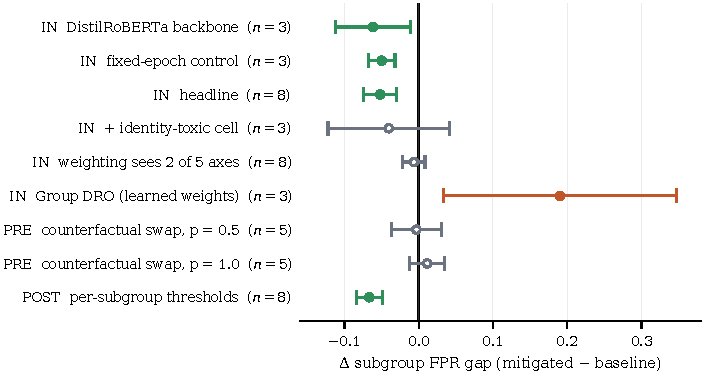
\includegraphics[width=\columnwidth]{fig_families}
\caption{Change in the subgroup FPR gap for every configuration, with the paired
$95\%$ confidence interval. A filled marker means the interval excludes zero.
Green is a significant improvement, orange a significant deterioration, grey
inconclusive. \textsc{in}, \textsc{pre} and \textsc{post} mark the intervention
point. Three-seed families carry a direction and an interval but no significance
claim; their sign test cannot fall below $0.25$.}
\label{fig:families}
\end{figure}

\begin{table*}[t]
\caption{Every configuration on the three axes. Only the eight-seed rows carry a
significance claim. A safety tax is printed only where the gap change itself
excludes zero; elsewhere the ratio would describe a near-zero denominator.}
\label{tab:families}
\centering
\small
\begin{tabular}{llrrrlcrrr}
\toprule
Stage & Configuration & $n$ & $\Delta$ gap & sd & 95\% CI & Sign & $\Delta$ F1 & $\Delta$ FNR & Tax \\
\midrule
\textsc{in} & loss reweighting (headline) & 8 & $-0.0520$ & $0.0266$ & $[-0.0742,\,-0.0297]$ & 8/8 & $-0.0128$ & $+0.1138$ & $2.19$ \\
\textsc{in} & reweighting, fixed epoch & 3 & $-0.0500$ & $0.0072$ & $[-0.0680,\,-0.0321]$ & 3/3 & $-0.0111$ & $+0.1306$ & $2.61$ \\
\textsc{in} & reweighting, DistilRoBERTa & 3 & $-0.0613$ & $0.0204$ & $[-0.1120,\,-0.0107]$ & 3/3 & $-0.0168$ & $+0.1526$ & $2.49$ \\
\textsc{in} & reweighting $+$ identity-toxic cell & 3 & $-0.0403$ & $0.0329$ & $[-0.1220,\,+0.0414]$ & 3/3 & $-0.0048$ & $+0.0698$ & -- \\
\textsc{in} & reweighting, 2 of 5 identity axes & 8 & $-0.0065$ & $0.0178$ & $[-0.0214,\,+0.0084]$ & 4/8 & $-0.0088$ & $+0.0830$ & -- \\
\textsc{in} & Group DRO, learned weights & 3 & $+0.1904$ & $0.0632$ & $[+0.0332,\,+0.3475]$ & 0/3 & $-0.0472$ & $-0.2308$ & -- \\
\addlinespace
\textsc{pre} & counterfactual swap, $p=0.5$ & 5 & $-0.0031$ & $0.0274$ & $[-0.0371,\,+0.0309]$ & 4/5 & $-0.0014$ & $-0.0016$ & -- \\
\textsc{pre} & counterfactual swap, $p=1.0$ & 5 & $+0.0114$ & $0.0192$ & $[-0.0124,\,+0.0352]$ & 1/5 & $-0.0069$ & $+0.0450$ & -- \\
\addlinespace
\textsc{post} & per-subgroup thresholds & 8 & $-0.0664$ & $0.0213$ & $[-0.0842,\,-0.0486]$ & 8/8 & $-0.0128$ & $+0.1183$ & $1.78$ \\
\bottomrule
\end{tabular}

\end{table*}

Reweighting works, and works on both backbones---on DistilRoBERTa the baseline
gap is \emph{larger} ($0.0866$ vs.\ $0.0767$ at seed $42$) although the model is
better on every quality metric, and the mitigation is more effective there, so
the phenomenon is not an artefact of one pretrained model.

The fixed-epoch control reproduces the effect at $-0.0500$ and collapses its
spread. Compared like for like on the same three seeds, the standard deviation of
the per-seed difference falls from $0.0427$ to $0.0072$, a factor of $5.9$. The
two arms do not peak on the same epoch---across those seeds the baseline was kept
at epoch $1,1,2$ and the mitigated arm at $2,2,2$---so the kept models differed in
more than the weight vector. Removing that difference leaves the effect intact
and locates most of the variance in checkpoint selection rather than in the
mitigation.

\subsection{The mechanism}
\label{sec:mechanism}
Fig.~\ref{fig:mechanism} shows why the disparity exists. Across the reportable
subgroups, a group's toxic rate on the test split predicts the model's FPR on
that group almost perfectly. Over the eight headline seeds the baseline slope is
$0.4405$ with $r = 0.9043$; the mitigated slope is $0.2310$ with $r = 0.9098$.
The intervention \textbf{flattens the line by $44.6\%$ and does not break it}: the
residual fit is just as tight. The model is not ``prejudiced'' against groups; it
has learned a conditional probability from the training distribution and applies
it as a prior to individual benign comments.

\begin{figure}[t]
\centering
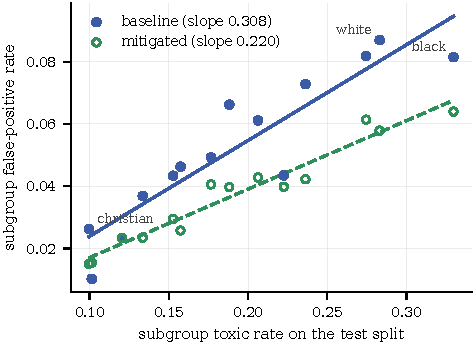
\includegraphics[width=\columnwidth]{fig_mechanism}
\caption{Subgroup false-positive rate against the subgroup's toxic rate on the
test split, seed $42$, over the $14$ reportable subgroups. Lines are
least-squares fits drawn only across the range their own data covers. Over the
eight seeds the slopes are $0.4405 \rightarrow 0.2310$, a $44.6\%$ flattening,
with $r = 0.9043 \rightarrow 0.9098$.}
\label{fig:mechanism}
\end{figure}

Table~\ref{tab:mechanism} fits the same regression in every configuration. Two
facts follow. The baseline slope is $0.44$--$0.48$ and the baseline correlation
$0.885$--$0.925$ \emph{everywhere}, which makes the shortcut the most reproducible
observation in the study. And the slope change does not track the gap change:
Fig.~\ref{fig:slope} shows two configurations that move the shortcut a long way
without closing the gap at all.

\begin{table*}[t]
\caption{The shortcut regression $\mathrm{FPR}_k = \beta\, t_k + c$, where $t_k$
is subgroup $k$'s toxic rate, fitted over the reportable subgroups in every
configuration. ``Gap closes?'' is taken from Table~\ref{tab:families}: yes only
where the paired interval excludes zero in the fair direction.}
\label{tab:mechanism}
\centering
\small
\begin{tabular}{lrrrrrc}
\toprule
Configuration & $n$ & Baseline slope & $r$ & Mitigated slope & Change & Gap closes? \\
\midrule
reweighting, DistilRoBERTa & 3 & $0.467$ & $0.916$ & $0.189$ & $-59.0$\% & yes \\
reweighting, fixed epoch & 3 & $0.442$ & $0.887$ & $0.219$ & $-50.4$\% & yes \\
loss reweighting (headline) & 8 & $0.441$ & $0.904$ & $0.231$ & $-44.6$\% & yes \\
counterfactual swap, $p=1.0$ & 5 & $0.466$ & $0.885$ & $0.319$ & $-30.9$\% & no \\
reweighting $+$ identity-toxic cell & 3 & $0.481$ & $0.925$ & $0.323$ & $-27.7$\% & no \\
counterfactual swap, $p=0.5$ & 5 & $0.466$ & $0.885$ & $0.424$ & $-7.6$\% & no \\
reweighting, 2 of 5 identity axes & 8 & $0.440$ & $0.904$ & $0.403$ & $-4.7$\% & no \\
Group DRO, learned weights & 3 & $0.480$ & $0.924$ & $1.447$ & $+224.4$\% & no \\
\bottomrule
\end{tabular}

\end{table*}

\begin{figure}[t]
\centering
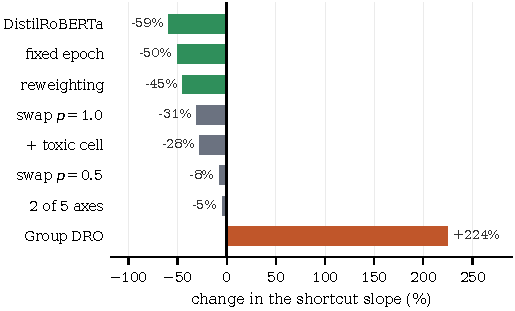
\includegraphics[width=\columnwidth]{fig_slope}
\caption{How far each configuration moves the shortcut slope. Green marks the
configurations that also close the FPR gap. The two grey bars at $-31\%$ and
$-28\%$ move the mechanism substantially \emph{without} closing the gap, and
Group DRO makes the shortcut three times steeper.}
\label{fig:slope}
\end{figure}

\subsection{Is the gain only a threshold shift?}
The first objection to any parity result of this kind is that the mitigated model
simply flags less. We test it directly: for each of the mitigated model's
operating points we interpolate the baseline's gap \emph{at the same global
false-positive rate}, and compare there. Points outside the baseline's measured
range are reported as non-comparable and excluded rather than clamped.

Over the eight seeds this yields $36$ comparable points. The mitigated model has
a smaller gap at $33$ of them ($91.7\%$), with a mean reduction of $23.9\%$ and a
median of $26.0\%$. Three points go the other way, all at high thresholds in
seeds $47$ and $49$ ($-14.6\%$, $-3.2\%$, $-0.2\%$). The effect therefore
survives matching at almost every operating point but not at all of them, which
closes the objection while reporting the exceptions.

Relatedly, the mitigated model's parity depends far less on where the operator
sets the dial: across $\tau \in [0.3, 0.7]$ the baseline's gap spans $0.1621$ and
the mitigated model's $0.0425$, $3.8\times$ narrower. For a deployed system whose
threshold is retuned continually, that stability is a practical result in its own
right.

Finally, direction. Because the gap is $\max - \min$, it falls both when the
worst-off subgroup improves (\emph{levelling up}) and when the best-off one
deteriorates (\emph{levelling down}), and only the first is a fairness gain. Over
the eight headline seeds the closure is levelling up in six and mixed in two.
By contrast Group DRO levels down in $3/3$ and counterfactual swapping in $4/5$.

\subsection{Counterfactual augmentation: a dose-response null}
\label{sec:cda}
At three seeds, counterfactual swapping looked like a small win. At five it is
$-0.0031$ with an interval spanning zero (Table~\ref{tab:families}); the earlier
verdicts were a small-sample artefact. Doubling the dose settles it. At
$p = 1.0$, every identity mention in training is randomised, and the gap moves
the \emph{wrong} way ($+0.0114$, improving in $1/5$ seeds). \textbf{A method whose
effect does not grow with its dose is not doing what its mechanism claims.}

The reason is sharper than ``it does nothing'', and it is the most useful negative
result in the paper. At $p = 1.0$ the augmentation \emph{demonstrably works}: the
shortcut regression flattens by $30.9\%$ (Fig.~\ref{fig:slope}), so the model
measurably stops using the identity token to predict toxicity. The disparity
survives anyway. \textbf{Removing the lexical shortcut is not sufficient to remove
the disparity}---the token was never the whole cause. The threshold-free metrics
agree: BPSN moves by $-0.0026$ at $p = 0.5$ and $-0.0012$ at $p = 1.0$, which is
nothing at either dose.

This also explains why reweighting succeeds where swapping does not. Reweighting
flattens the same slope by $44.6\%$ \emph{and} closes the gap, because it prices
the whole identity-bearing region of input space rather than editing one token
inside it.

\subsection{Group DRO: the objective refutes itself}
\label{sec:dro}
Group DRO learns a weight vector over the same four cells we weight by hand,
which makes it our method with the one human decision removed. It reached outcome
\textbf{D} in $3/3$ seeds: the FPR gap became $2.6\times$ worse
($0.1153 \rightarrow 0.3056$) while subgroup FNR fell by $0.2308$. This is not a
collapse but a real, well-behaved model that travelled the frontier backwards.

Table~\ref{tab:dro} shows why. The optimiser zeroed the easy majority cell and
split its weight almost evenly between the \emph{two} identity cells---which is
essentially the configuration we tested by hand and rejected, rediscovered
without a human choosing it, and it reproduced that configuration's failure mode
amplified.

\begin{table}[t]
\caption{What Group DRO learned, against what we assumed. The learned column
gives the final weight vector for seeds $42/43/44$; our static vector is shown
normalised to sum to one for comparability.}
\label{tab:dro}
\centering
\small
\begin{tabular}{lrl}
\toprule
Cell & Ours & Group DRO, per seed \\
\midrule
background, non-toxic & $0.143$ & 0.000 / 0.000 / 0.000 \\
background, toxic & $0.143$ & 0.142 / 0.146 / 0.163 \\
identity, non-toxic & $0.571$ & 0.451 / 0.424 / 0.446 \\
identity, toxic & $0.143$ & 0.407 / 0.431 / 0.391 \\
\bottomrule
\end{tabular}

\end{table}

A worst-group objective \emph{cannot} find our solution, and the reason is
structural: the identity-bearing toxic cell also carries high loss, so any
worst-group criterion necessarily raises it.

\subsection{Does the effect reach groups it was never paid to see?}
\label{sec:heldout}
If the intervention teaches ``identity-bearing language deserves more care'' it
should transfer; if it teaches ``these particular tokens are expensive'' it
should not. We test this by computing the weighting's identity signal from gender
and religion only, while the audit continues to measure every subgroup
(Table~\ref{tab:heldout}).

\begin{table*}[t]
\caption{The held-out experiment over eight seeds. \texttt{main} is shown under
the same axis split, which removes the dose confound: the weighted axes improve
by essentially the same amount in both runs, so the movement on the untouched
axes is transfer rather than a diluted dose.}
\label{tab:heldout}
\centering
\small
\setlength{\tabcolsep}{4pt}
\begin{tabular}{lrrrlcrc}
\toprule
Axis bucket & $n$ & mean $\Delta$ FPR & sd & 95\% CI & Seeds & $p$ & Subgroup obs. \\
\midrule
\texttt{heldout}: weighted axes (gender, religion) & 8 & $-0.0277$ & $0.0162$ & $[-0.0412,\,-0.0142]$ & 8/8 & $0.0078$ & 56/58 \\
\texttt{heldout}: held-out axes (race, orient., disab.) & 8 & $-0.0161$ & $0.0185$ & $[-0.0315,\,-0.0007]$ & 6/8 & $0.2891$ & 36/56 \\
\addlinespace
\texttt{main}: same weighted axes & 8 & $-0.0258$ & $0.0124$ & $[-0.0362,\,-0.0155]$ & 8/8 & $0.0078$ & 56/58 \\
\texttt{main}: same held-out axes & 8 & $-0.0392$ & $0.0193$ & $[-0.0553,\,-0.0230]$ & 8/8 & $0.0078$ & 55/56 \\
\bottomrule
\end{tabular}

\end{table*}

The intervention transfers at about $58\%$ strength. The confound this could have
had is measured and absent: the weighted axes improve by $-0.0277$ here against
$-0.0258$ for the same axes in the full run, so narrowing the weighting did not
weaken it where it still applied.

Two qualifications must travel with this result. First, the paired interval
excludes zero only just, and a sign test on $6/8$ does not ($p = 0.29$); we call
it suggestive, not established. Second, \textbf{the transfer is a level shift, not
a slope change}: this configuration lowers macro FPR in $8/8$ seeds but flattens
the shortcut by only $4.7\%$, against $44.6\%$ for the full weighting. Teaching
the loss about two axes makes the model more cautious about identity-bearing
language in general without re-ordering the groups relative to their toxic rate.
That is also why its FPR \emph{gap} appears flat while almost every subgroup
improves: the gap is $\max - \min$, and the max is a held-out group.

\subsection{Ablation and the two mirror controls}
\label{sec:ablation}
Table~\ref{tab:ablation} sweeps $\alpha$ and reports the \texttt{class} control.
Parity gains flatten after $\alpha = 4$ while the safety cost keeps climbing
(Fig.~\ref{fig:alpha}), so the pre-registered default sits at the knee rather
than at a tuned optimum. No arm collapsed at any $\alpha$, including $10$.

\begin{table*}[t]
\caption{Ablation on the headline configuration, three seeds. The
\texttt{class} arm is the control that answers whether ordinary imbalance
handling would have produced the same effect. The flag rate is printed beside
every arm because an arm can post a small gap simply by flagging almost nothing.}
\label{tab:ablation}
\centering
\small
\begin{tabular}{llrrrrr}
\toprule
Scheme & Arm & FPR gap & macro FPR & macro-F1 & subgroup FNR & Flag rate \\
\midrule
subgroup & $\alpha = 1$ (= baseline) & $0.1152$ & $0.0747$ & $0.8028$ & $0.4183$ & $0.1050$ \\
subgroup & $\alpha = 2$ & $0.0750$ & $0.0461$ & $0.7958$ & $0.5026$ & $0.0917$ \\
subgroup & \textbf{$\alpha = 4$} & $0.0508$ & $0.0355$ & $0.7900$ & $0.5515$ & $0.0846$ \\
subgroup & $\alpha = 6$ & $0.0501$ & $0.0304$ & $0.7861$ & $0.5747$ & $0.0817$ \\
subgroup & $\alpha = 10$ & $0.0443$ & $0.0254$ & $0.7825$ & $0.6020$ & $0.0787$ \\
\addlinespace
class & inverse class frequency & $0.3005$ & $0.2157$ & $0.7776$ & $0.2039$ & $0.1770$ \\
\bottomrule
\end{tabular}

\end{table*}

\begin{figure}[t]
\centering
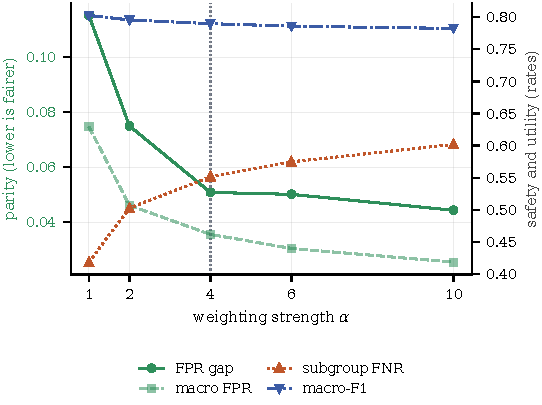
\includegraphics[width=\columnwidth]{fig_alpha}
\caption{The three axes as the weighting strength rises, three seeds. Parity
gains flatten after the dotted line---the pre-registered $\alpha = 4$---while the
safety cost keeps climbing. Macro FPR is shown alongside the FPR gap because the
gap depends on only two subgroups and is the noisier of the two.}
\label{fig:alpha}
\end{figure}

The \texttt{class} control is decisive. Weighting by inverse class frequency,
which knows nothing about identity, makes the FPR gap $2.6\times$ \emph{worse}
($0.1152 \rightarrow 0.3005$) while flagging $17.7\%$ of everything. Ordinary
imbalance handling is not a substitute for identity-aware weighting; it is the
opposite of one.

The second control is its mirror. Isolating the identity-bearing \emph{toxic}
cell moves the FPR gap from $0.0767$ to $0.1374$ (worse) while macro FNR falls
from $0.4744$ to $0.3374$ (better)---the exact reflection of the \texttt{class}
result. Together the two controls turn ``we observed a trade-off'' into ``the two
axes are structurally coupled in this weighting family, and we demonstrated it
from both sides''.

\subsection{Threshold-free confirmation}
Table~\ref{tab:tf} reports the Borkan metrics, which require no threshold at all.
For the headline configuration BPSN---the threshold-free analogue of our FPR
gap---rises from $0.8751$ to $0.8865$, while BNSP, which measures
under-protection, falls from $0.9413$ to $0.9244$. Two independent metric
families therefore agree with the thresholded result: the parity gain is real and
so is the safety cost, and neither conclusion depends on $\tau = 0.5$.

\begin{table*}[t]
\caption{Threshold-free metrics of Borkan et al.~\cite{borkan2019}, averaged over
each configuration's seeds. BPSN is the threshold-free analogue of the FPR gap;
BNSP measures under-protection.}
\label{tab:tf}
\centering
\small
\begin{tabular}{lrrrrrr}
\toprule
Configuration & $n$ & BPSN base & BPSN mit. & $\Delta$ BPSN & $\Delta$ BNSP & $\Delta$ AUC \\
\midrule
loss reweighting (headline) & 8 & $0.8751$ & $0.8865$ & $+0.0114$ & $-0.0169$ & $-0.0061$ \\
reweighting, DistilRoBERTa & 3 & $0.8788$ & $0.8941$ & $+0.0153$ & $-0.0170$ & $-0.0046$ \\
counterfactual swap, $p=0.5$ & 5 & $0.8738$ & $0.8712$ & $-0.0026$ & $-0.0003$ & $-0.0015$ \\
counterfactual swap, $p=1.0$ & 5 & $0.8738$ & $0.8726$ & $-0.0012$ & $-0.0072$ & $-0.0042$ \\
Group DRO, learned weights & 3 & $0.8746$ & $0.8844$ & $+0.0098$ & $-0.0166$ & $-0.0070$ \\
reweighting, 2 of 5 identity axes & 8 & $0.8751$ & $0.8770$ & $+0.0019$ & $-0.0157$ & $-0.0057$ \\
\bottomrule
\end{tabular}

\end{table*}

One caveat deserves its own sentence, because it separates two claims that are
easily conflated. \textbf{Group DRO improves BPSN} ($+0.0098$) while its
thresholded FPR gap gets $2.6\times$ worse. Threshold-free parity and parity at a
fixed operating point are different claims, and Group DRO is the case that
separates them: it shifts the operating point so far that a better ranking still
produces a much worse gap at $\tau = 0.5$.

\subsection{Post-processing, and the cost it hides}
Per-subgroup thresholds---fitted on validation, scored on test, with $13$ or $14$
of the $14$ reportable subgroups receiving one---reduce the gap by $0.0664$ in
$8/8$ seeds (Table~\ref{tab:families}). That is a \emph{larger} parity gain than
retraining, at no GPU cost at all.

It must never be quoted without the sentence that follows. A per-group threshold
needs the identity annotation of a comment \textbf{at inference time}. The
training-time methods consume identity annotations once, during training, and
never again. In a deployed moderation system the post-processing method would
require inferring or storing the demographic attributes of the text being
judged---which is both a practical obstacle and an ethical one. The method wins
on parity and loses on deployability, and both halves are the result.

\subsection{What the false positives actually are}
\label{sec:coding}
Aggregate rates say how much; they do not say what. We drew a \emph{uniform
random} sample of $60$ of the baseline's $1{,}025$ identity-bearing false
positives---deliberately not the most confident ones, whose composition is the
composition of the confident tail rather than of the errors---and read and coded
every one along two axes: whom the hostility is aimed at, and whether the
dataset's non-toxic label is defensible (Table~\ref{tab:coding}).

\begin{table*}[t]
\caption{Manual coding of a uniform random sample of $60$ identity-bearing false
positives from the baseline model. ``Label arguable'' counts comments a
reasonable annotator could have called toxic.}
\label{tab:coding}
\centering
\small
\begin{tabular}{lrrrl}
\toprule
Category & $n$ & \% & Label arguable & What the comment is \\
\midrule
\texttt{hostility\_not\_group\_directed} & 21 & $35.0$ & 11 & hostile, but aimed at a person, party or ideology \\
\texttt{group\_directed\_derogation} & 16 & $26.7$ & 16 & genuinely derogatory towards the group \\
\texttt{counter\_speech} & 12 & $20.0$ & 0 & argues \emph{against} bigotry \\
\texttt{identity\_topic\_neutral} & 7 & $11.7$ & 0 & neutral mention, no hostility at all \\
\texttt{quoted\_hostility} & 4 & $6.7$ & 0 & quotes hostile speech in order to criticise it \\
\bottomrule
\end{tabular}

\end{table*}

Two numbers change how the rest of the paper should be read.

\textbf{$27$ of $60$ ($45\%$) are comments a reasonable annotator could have
called toxic.} Nearly half of what the metrics call a false positive is annotator
disagreement rather than model error. Stating this does not weaken the study's
claim---the claim is about a controlled difference between two arms measured
identically---but it does bound what the absolute FPR means.

\textbf{In the other half the model penalises exactly the text that should be
protected.} Counter-speech, quoted hostility and plain neutral mention together
are $23/60$ ($38\%$): text that argues against bigotry, quotes it in order to
criticise it, or merely names a group. For a moderation system this is the worst
error type available, because it silences the speech the policy exists to
protect.

We also measured our own regular-expression triage against the human coding and
report that it is weak: it recovers $3$ of the $12$ true counter-speech comments
($25\%$ recall) at $75\%$ precision. Every category count in this paper therefore
comes from the coded sample, never from the heuristic columns.

\subsection{Who is affected}
Fig.~\ref{fig:fpr} and Fig.~\ref{fig:fnr} give the per-subgroup picture that the
aggregates compress. Twelve of the $14$ reportable subgroups improve on FPR;
\texttt{asian} is unchanged---its false-positive rate is identical in both arms
to six decimal places---and \texttt{atheist} gets \emph{worse}
($0.0103 \rightarrow 0.0154$, $+50\%$). The most strongly supported single claim
in the study is that a benign comment mentioning \texttt{white} is flagged
$3.3\times$ more often than one mentioning \texttt{christian}
($0.0870$ vs.\ $0.0262$; thousands of rows each, disjoint Wilson intervals).
On the safety side, all nine subgroups entitled to an FNR claim get worse, and
strikingly evenly---between $7.5$ and $10.2$ points---which indicates that the
intervention shifts the model's overall operating point rather than harming any
particular group.

\begin{figure}[t]
\centering
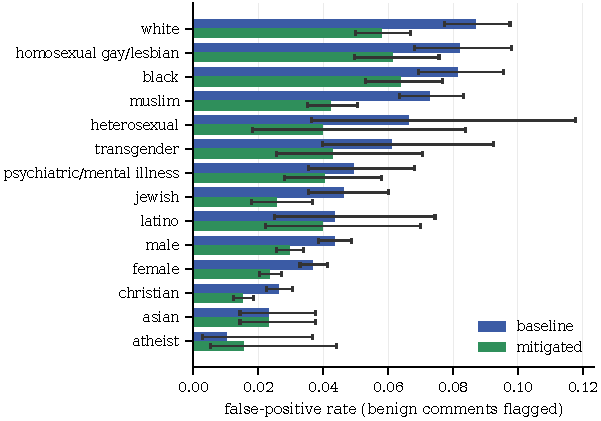
\includegraphics[width=\columnwidth]{fig_fpr_subgroup}
\caption{False-positive rate by subgroup with Wilson $95\%$ intervals, seed $42$,
for the $14$ subgroups clearing the FPR support floor. Twelve improve,
\texttt{asian} is unchanged, and \texttt{atheist}---the smallest and best-served
group---gets worse.}
\label{fig:fpr}
\end{figure}

% [b] rather than [t]: the two per-subgroup panels are single-column floats and
% would otherwise be typeset side by side in the same horizontal band, which
% reads as one wide figure that has been split rather than as two figures.
\begin{figure}[b]
\centering
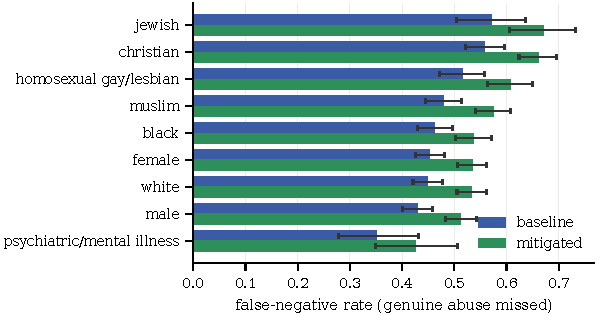
\includegraphics[width=\columnwidth]{fig_fnr_subgroup}
\caption{False-negative rate by subgroup, seed $42$, for the $9$ subgroups
clearing the FNR support floor. Every one is worse under the mitigation. This is
the safety cost the headline table prices at $2.19$.}
\label{fig:fnr}
\end{figure}

\subsection{Integrity and leakage}
Table~\ref{tab:integrity} records the checks that make the paired comparisons
legitimate: within every seed, all runs share one partition and one GPU, and no
model collapsed.

The split is by row rather than by text, and the corpus contains repeated
comments, so between $0.98\%$ and $1.11\%$ of test rows occur verbatim in
training. We measured the consequence instead of arguing about it: removing those
rows and recomputing both arms shifts the mitigation effect by at most $0.0032$
and by $+0.0005$ on average. Both arms share one partition, so both are inflated
identically and the paired difference carries no contamination; only the absolute
figures are mildly inflated, and now by a measured amount.

\begin{table*}[t]
\caption{Per-seed integrity checks over all $38$ runs. A single split fingerprint
per seed is what makes the configurations comparable with each other and not only
each with its own baseline.}
\label{tab:integrity}
\centering
\small
\begin{tabular}{rrlccrr}
\toprule
Seed & Runs & Split fingerprint & One partition & One GPU & Collapsed & Dup.\ \% \\
\midrule
42 & 8 & \texttt{798dd7cc3c01ef5a} & yes & yes & none & $1.09$ \\
43 & 8 & \texttt{39a5c590e88707e2} & yes & yes & none & $1.10$ \\
44 & 8 & \texttt{41cd4a89437acdbd} & yes & yes & none & $1.00$ \\
45 & 4 & \texttt{435d5de1b711cd7c} & yes & yes & none & $0.98$ \\
46 & 4 & \texttt{3a7fa90ef16c138c} & yes & yes & none & $1.06$ \\
47 & 2 & \texttt{8a1a4c881597f3e9} & yes & yes & none & $1.11$ \\
48 & 2 & \texttt{c32c2cd9766f0580} & yes & yes & none & $0.98$ \\
49 & 2 & \texttt{1265af7b462697f9} & yes & yes & none & $1.02$ \\
\bottomrule
\end{tabular}

\end{table*}

%==============================================================================
\section{Discussion}
%==============================================================================

\subsection{The finding, stated plainly}
The disparity is not a bug in one model. It is an almost linear function of the
training distribution, reproducible at $r \geq 0.885$ across two backbones and
eight configurations. It can be reduced---reliably, and by a measurable
amount---but in this weighting family it cannot be reduced for free, and the
price is paid in exactly the currency a moderation system cares about most.

The more useful finding is \emph{why} only one of our interventions worked. Three
independent lines converge on it. Ordinary class weighting makes the gap
$2.6\times$ worse. Weighting the identity-toxic cell alone makes the gap worse
and safety better. Group DRO, which contains no human choice whatsoever, learns
almost exactly the second of those and reproduces its failure amplified. The
parity gain requires an \emph{asymmetric} weighting of the identity-bearing
non-toxic cell alone; any objective that also raises the identity-bearing toxic
cell travels the same frontier backwards. A worst-group objective cannot find our
solution, because the identity-toxic cell also carries high loss.

The held-out experiment (Section~\ref{sec:heldout}) qualifies how that mechanism
should be described. What the weighting teaches does generalise to axes it never
saw, but as a \emph{level shift} rather than a change of ordering: the model
becomes more cautious about identity-bearing language in general without
re-ranking the groups against their toxic rate. The shortcut and the disparity
are related but not identical---which is the conclusion the augmentation dose
experiment reaches from the opposite direction, and the two agreeing is the
strongest evidence we have for it.

\subsection{What this means for a deployed system}
An operator choosing among these methods faces a choice we can now state
concretely. Post-processing gives the largest parity gain for no training cost
but requires demographic information at inference time. Reweighting gives a
slightly smaller gain, needs identity annotations only during training, and
additionally makes parity far less sensitive to the threshold---a real operational
advantage, since deployed thresholds move. Counterfactual augmentation, on this
corpus, buys nothing at either dose. And every method that reduces the FPR gap in
our study increases missed abuse; an operator who cannot accept that increase
should not expect this family of methods to help.

%==============================================================================
\section{Limitations}
%==============================================================================

\begin{itemize}
\item \textbf{Absolute parity improved; the relative parity of the
      highest-support pair did not.} The \texttt{white}/\texttt{christian} ratio
      goes $3.32\times \rightarrow 3.83\times$. We state it that precisely
      because the worst/best ratio over all $14$ subgroups moves the other way
      ($8.48\times \rightarrow 4.23\times$); a flat claim in either direction
      would be false.
\item \textbf{One subgroup got worse.} \texttt{atheist} rose $50\%$ in relative
      terms from a small base, and \texttt{asian} did not move.
\item \textbf{Part of the measured FPR is annotator disagreement}, not model
      error---$45\%$ of a random sample, with a Wilson interval of roughly
      $[33\%, 58\%]$ at $n = 60$ (Section~\ref{sec:coding}).
\item \textbf{The coding has one coder}, so we report no inter-annotator
      agreement; a second coder on a subset would fix this cheaply, and only the
      baseline arm was coded.
\item \textbf{Support is uneven.} $14$ of $24$ subgroups can carry a parity claim
      and only $9$ a safety claim under the separate floors of
      Section~\ref{sec:guards}; \texttt{other\_disability} has no test rows at
      all, so audits report $23$ subgroups rather than $24$.
\item \textbf{Only two of the eight configurations reach eight seeds.} Four have
      three and two have five, which supports a direction and an interval but no
      significance claim. We print their sign test anyway, at its floor of
      $0.25$, so that $3/3$ is never mistaken for evidence.
\item \textbf{The worst-affected subgroup changes} between arms
      (\texttt{white}~$\rightarrow$~\texttt{black}), and we do not explain why.
\item \textbf{Attribution is not causation.} Integrated
      Gradients~\cite{sundararajan2017} measures local input sensitivity along a
      path from a baseline input; we report the identity-token attribution share
      ($0.1164 \rightarrow 0.1001$, $-14\%$ over $20$ paired explanations) as
      supporting analysis only, never as evidence about how the model reasons.
\item \textbf{Scope.} One corpus, one language, one architecture family, and
      binary coarse identity categories that real identity does not respect.
\end{itemize}

%==============================================================================
\section{Conclusion and Future Work}
%==============================================================================

We compared bias mitigations at all three points of the pipeline on one corpus
under one recipe, with replication and pre-registered outcomes. Identity-aware
loss reweighting reduces the subgroup FPR gap by $0.0520$ over eight seeds
($p = 0.0078$) and flattens the shortcut that produces the gap by $44.6\%$, at a
cost of $2.19$ points of missed abuse per point of gap closed. Per-subgroup
thresholds do better on parity and worse on deployability. Counterfactual
augmentation does nothing at either dose---while measurably removing the lexical
shortcut, which shows the shortcut and the disparity are not the same thing. The
learned-weight version of our own objective moves the gap backwards and, in
doing so, identifies the asymmetry that makes the working method work.

Three directions follow. A second coder on the error sample would put an
agreement statistic on the $45\%$ figure. Extending the held-out experiment to
more axis splits would turn a suggestive transfer result into a tested one. And
the frontier itself invites a direct attack: the coupling we document is a
property of a weighting family, and whether an intervention outside that family
can close the gap without paying in safety is, on this evidence, still open.

%==============================================================================
\section*{Tools and Acknowledgements}
%==============================================================================

AI assistance (large-language-model coding assistants) was used during this
project for: refactoring and documenting source code; drafting and copy-editing
the English prose of this report; searching and summarising related literature;
and generating boilerplate for plotting and table export. All experimental design
decisions, the pre-registration of the outcome thresholds, the choice of metrics,
controls and support floors, the manual error coding, and the interpretation of
every result reported here are the authors' own. No AI system was used to
generate, alter or select any experimental result. Every line of the released
code has been read by the authors, and each author is able to explain and defend
any part of the system.

We thank the teaching staff of the AI Academy for the shared A100 allocation and
for feedback on an earlier draft.

%==============================================================================
\balance
\begin{thebibliography}{99}

\bibitem{dixon2018}
L.~Dixon, J.~Li, J.~Sorensen, N.~Thain, and L.~Vasserman, ``Measuring and
mitigating unintended bias in text classification,'' in \emph{Proc.\ AAAI/ACM
Conf.\ AI, Ethics, and Society (AIES)}, New Orleans, LA, USA, 2018, pp.\ 67--73.

\bibitem{borkan2019}
D.~Borkan, L.~Dixon, J.~Sorensen, N.~Thain, and L.~Vasserman, ``Nuanced metrics
for measuring unintended bias with real data for text classification,'' in
\emph{Companion Proc.\ World Wide Web Conf.\ (WWW)}, San Francisco, CA, USA,
2019, pp.\ 491--500.

\bibitem{sap2019}
M.~Sap, D.~Card, S.~Gabriel, Y.~Choi, and N.~A. Smith, ``The risk of racial bias
in hate speech detection,'' in \emph{Proc.\ 57th Annu.\ Meeting Assoc.\ for
Computational Linguistics (ACL)}, Florence, Italy, 2019, pp.\ 1668--1678.

\bibitem{park2018}
J.~H. Park, J.~Shin, and P.~Fung, ``Reducing gender bias in abusive language
detection,'' in \emph{Proc.\ Conf.\ Empirical Methods in Natural Language
Processing (EMNLP)}, Brussels, Belgium, 2018, pp.\ 2799--2804.

\bibitem{garg2023}
T.~Garg, S.~Masud, T.~Suresh, and T.~Chakraborty, ``Handling bias in toxic speech
detection: A survey,'' \emph{ACM Comput.\ Surv.}, vol.\ 55, no.\ 13s, art.\ 264,
pp.\ 1--32, 2023.

\bibitem{gupta2025}
S.~Gupta, V.~Kovatchev, A.~Das, M.~De-Arteaga, and M.~Lease, ``Finding Pareto
trade-offs in fair and accurate detection of toxic speech,'' \emph{Information
Research}, vol.\ 30, iConf., pp.\ 123--141, 2025.

\bibitem{garg2019}
S.~Garg, V.~Perot, N.~Limtiaco, A.~Taly, E.~H. Chi, and A.~Beutel,
``Counterfactual fairness in text classification through robustness,'' in
\emph{Proc.\ AAAI/ACM Conf.\ AI, Ethics, and Society (AIES)}, Honolulu, HI, USA,
2019, pp.\ 219--226.

\bibitem{lu2024}
J.~Lu, B.~Xu, X.~Zhang, K.~Liu, D.~Zhang, L.~Yang, and H.~Lin, ``Take its
essence, discard its dross! Debiasing for toxic language detection via
counterfactual causal effect,'' 2024, arXiv:2406.00983.

\bibitem{zhang2018}
B.~H. Zhang, B.~Lemoine, and M.~Mitchell, ``Mitigating unwanted biases with
adversarial learning,'' in \emph{Proc.\ AAAI/ACM Conf.\ AI, Ethics, and Society
(AIES)}, New Orleans, LA, USA, 2018, pp.\ 335--340.

\bibitem{sagawa2020}
S.~Sagawa, P.~W. Koh, T.~B. Hashimoto, and P.~Liang, ``Distributionally robust
neural networks for group shifts: On the importance of regularization for
worst-case generalization,'' in \emph{Proc.\ Int.\ Conf.\ Learning
Representations (ICLR)}, 2020.

\bibitem{hardt2016}
M.~Hardt, E.~Price, and N.~Srebro, ``Equality of opportunity in supervised
learning,'' in \emph{Advances in Neural Information Processing Systems (NIPS)},
Barcelona, Spain, 2016, pp.\ 3315--3323.

\bibitem{sanh2019}
V.~Sanh, L.~Debut, J.~Chaumond, and T.~Wolf, ``DistilBERT, a distilled version of
BERT: smaller, faster, cheaper and lighter,'' 2019, arXiv:1910.01108.

\bibitem{liu2019}
Y.~Liu, M.~Ott, N.~Goyal, J.~Du, M.~Joshi, D.~Chen, O.~Levy, M.~Lewis,
L.~Zettlemoyer, and V.~Stoyanov, ``RoBERTa: A robustly optimized BERT pretraining
approach,'' 2019, arXiv:1907.11692.

\bibitem{jigsaw2019}
cjadams, D.~Borkan, inversion, J.~Sorensen, L.~Dixon, L.~Vasserman, and
N.~Thain, ``Jigsaw unintended bias in toxicity classification,'' Kaggle
competition, 2019. Dataset licensed CC0 1.0. [Online]. Available:
\url{https://www.kaggle.com/c/jigsaw-unintended-bias-in-toxicity-classification}

\bibitem{wolf2020}
T.~Wolf \emph{et al.}, ``Transformers: State-of-the-art natural language
processing,'' in \emph{Proc.\ Conf.\ Empirical Methods in Natural Language
Processing: System Demonstrations}, 2020, pp.\ 38--45.

\bibitem{paszke2019}
A.~Paszke \emph{et al.}, ``PyTorch: An imperative style, high-performance deep
learning library,'' in \emph{Advances in Neural Information Processing Systems
(NeurIPS)}, 2019, pp.\ 8024--8035.

\bibitem{pedregosa2011}
F.~Pedregosa \emph{et al.}, ``Scikit-learn: Machine learning in Python,''
\emph{J.\ Machine Learning Research}, vol.\ 12, pp.\ 2825--2830, 2011.

\bibitem{wilson1927}
E.~B. Wilson, ``Probable inference, the law of succession, and statistical
inference,'' \emph{J.\ American Statistical Association}, vol.\ 22, no.\ 158,
pp.\ 209--212, 1927.

\bibitem{sundararajan2017}
M.~Sundararajan, A.~Taly, and Q.~Yan, ``Axiomatic attribution for deep
networks,'' in \emph{Proc.\ Int.\ Conf.\ Machine Learning (ICML)}, Sydney,
Australia, 2017, pp.\ 3319--3328.

\end{thebibliography}

\end{document}
